\documentclass[fleqn]{article}
%\textwidth=6in
%\textheight=9in
%\pagestyle{empty}
\usepackage{amsmath,amssymb,amsthm,ragged2e,siunitx,graphicx,multicol,wrapfig,mathtools,parskip}
\usepackage[margin=0.7in]{geometry}
\usepackage[T1]{fontenc}
\usepackage[utf8]{inputenc}
\usepackage[dvipsnames]{xcolor}
\usepackage[export]{adjustbox}
\newtheorem{thm}{{\sc Theorem}}[section]
\newtheorem{prop}[thm]{{\sc Proposition}}
\newtheorem{cor}[thm]{{\sc Corollary}}
\newtheorem{lem}[thm]{{\sc Lemma}}
\newtheorem{df}[thm]{{\sc Definition}}

\DeclarePairedDelimiter\ceil{\lceil}{\rceil}
\DeclarePairedDelimiter\floor{\lfloor}{\rfloor}

\DeclareMathOperator{\sech}{sech}
\DeclareMathOperator{\csch}{csch}

% automatically makes new paragraphs have no indent
\setlength{\parindent}{0pt}

% new command for underscore
\newcommand{\underscore}{\underline{\hspace{1cm}}}

% this is a command for the space between asterisk or plus and the problem statement
\newcommand{\gap}{\hspace{.25cm}}

\newcommand*\colvec[1]{\begin{bmatrix*}[r]#1\end{bmatrix*}} 

% Uncomment this to write vectors bolded 
\renewcommand{\vec}[1]{\boldsymbol{#1}}

% Uncomment this to write vectors bolded AND with arrow on top
\newcommand{\avec}[1]{\overrightarrow{\boldsymbol{#1}}}
% this notation has an arrow on top of vector which is redundant if it is bolded

% Uncomment this to write vectors unbolded with long arrow on top
% \renewcommand{\vec}[1]{\overrightarrow{#1}}

% this is a command for a coefficient matrix with right-aligned entries (good for aligning negative signs)
\newcommand{\mat}[1]{\begin{bmatrix*}[r]#1\end{bmatrix*}} 

% this is a command for a coefficient matrix with center-aligned entries (good for aligning negative signs)
\newcommand{\cmat}[1]{\begin{bmatrix*}[c]#1\end{bmatrix*}} 

% this is a command for a DETERMNINANT matrix with right-aligned entries (good for aligning negative signs) (ABSOLUTE VALUE BARS)
\newcommand{\vmat}[1]{\begin{vmatrix*}[r]#1\end{vmatrix*}} 

% this is a command for black squares (useful for pivots in matrices) when already in math mode (between $ signs)
\newcommand{\bsq}{\blacksquare}






%%  environment for AUGMENTED  matrices
\newenvironment{amatrix}[1]{%
  \left[\begin{array}{@{}*{#1}{r}|r@{}}
}{%
  \end{array}\right]
}


%%% new command for Augmented BAR alone (helpful for putting augmented bar somewhere in middle of matrix)
\newcommand\aug{\fboxsep=-\fboxrule\!\!\!\fbox{\strut}\!\!\!}

% define new color (i.e. pink)
\definecolor{mypink1}{rgb}{0.858, 0.188, 0.478}

% define new color (i.e. medium green)
\definecolor{MediumGreen}{rgb}{0.1, 0.8, 0.65}

% define new color (i.e. dark purple)
\definecolor{DarkPurple}{rgb}{0.6, 0, 0.6}

% this is a command for the size of headers
\newcommand{\header}[1]{\noindent{\Large \textcolor{mypink1}{\textbf{#1}}}}

% this is a command for the size of subheaders
\newcommand{\subheader}[1]{\noindent{\large \textcolor{red}{\textbf{#1}}}}

% this is a command for answers in RED on same line with a space between problem and answer
\newcommand{\sred}[1]{\hspace{1cm} \textcolor{red}{#1}}

% this is a command for answers in RED on same line with NO space between problem and answer
\newcommand{\red}[1]{\textcolor{red}{#1}}

% this is a command for answers in PURPLE on same line with NO space between problem and answer
\newcommand{\DarkPurple}[1]{\textcolor{DarkPurple}{#1}}

% this is a command for answers in GREEN on same line with NO space between problem and answer
\newcommand{\MediumGreen}[1]{\textcolor{MediumGreen}{#1}}

% this is a command for answers in BLUE on same line with a space between problem and answer
\newcommand{\sblue}[1]{\hspace{1cm} \textcolor{blue}{#1}}

% this is a command for answers in BLUE on same line with NO space between problem and answer
\newcommand{\blue}[1]{\textcolor{blue}{#1}}


% this is a command for defining EXAMPLES
\theoremstyle{definition}
\newtheorem{exmp}{Example}[section]




\begin{document}

\centerline{\Large \bf Math Seminar Template Notes}
\centerline{\large \bf Day 3 (More Induction)}
\vspace{\baselineskip}

%\noindent \underline{\hspace{18cm}}

\header{Day 3 (More Induction) } \\


\noindent\fbox{%
\parbox{\textwidth}{
\subheader{Overview} \\ 
%\vspace{0.25cm}
\textbf{\underline{Goals}} 
\begin{enumerate}
\item Recap what induction is and continue practicing this 
\item Find a flaw in an induction ``proof"
\item Explore how we can modify induction and make it stronger 
\end{enumerate}
\vspace{.25cm}
}}

\vspace{0.2cm}

\subheader{Induction Recap}

Suppose we are trying to show some statement, $P(n)$, is true for all integers $n \geq 1$. 

\vspace{.05cm}
	\hspace{1cm} $\displaystyle{ \Bigg( }$ e.g. $P(n)$ might be the statement $\displaystyle{1^2+2^2+3^2 + \ldots + n^2 = \frac{n(n+1)(2n+1)}{6} }$ $\displaystyle{ \Bigg) }$

\vspace{.25cm}
It's hard to show such statements using our earlier methods.

\vspace{.25cm}
%%%% something in a box
\noindent\fbox{%
\parbox{\textwidth}{\vspace{.25cm}
\textbf{Idea:} Represent, $P(1), P(2), P(3), \ldots $ using \textbf{dominoes}.  

%image centered
%%
\begin{center}
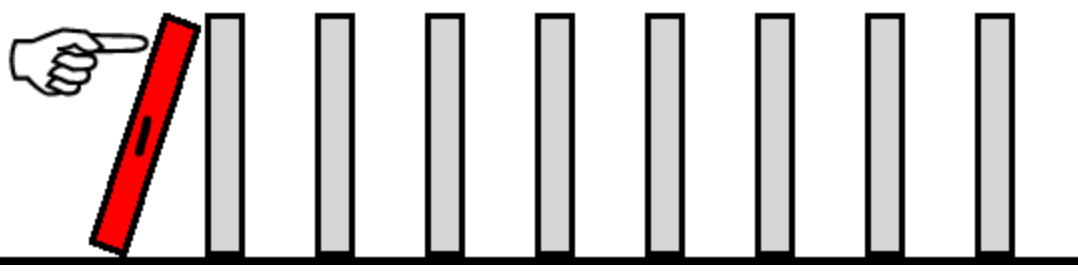
\includegraphics[scale=0.5]{InductionDominoes}
\end{center} 
% \vspace{-20pt}

Suppose we know the following: 

	\vspace{.2cm}
	\begin{enumerate}
	\item Domino $1$ falls

	\vspace{.25cm}
	\item If domino $k$ falls, then domino $k+1$ also falls (for any positive integer $k$)
	\end{enumerate}

\vspace{.25cm}
\textbf{Outcome:} Then, \underline{\hspace{2cm}} dominoes will fall!
\vspace{.25cm}   
}}
%%% end box



\vspace{.25cm}
%%%% something in a box
\noindent\fbox{%
\parbox{\textwidth}{\vspace{.25cm}
\hspace{5cm} \textbf{Principle of Mathematical Induction} 

\vspace{.25cm}
To prove a statement, $P(n)$, is true for all integers $n \geq 1$ ($n \in \mathbb{Z}^+$), using \textbf{induction}, there are 2 steps:

	\vspace{.25cm}
	\begin{enumerate}
	\item \textbf{(Base Step):} Show \underline{\hspace{1.5cm}} is true

	\vspace{.25cm}
	\item \textbf{(Inductive Step):} Assume \underline{\hspace{1.5cm}} is true for an arbitrary $k \in \mathbb{Z}^+$, and show this implies that \underline{\hspace{1.75cm}} is true. 

%	\vspace{.25cm}
%	\hspace{1cm} i.e. show $\underline{\hspace{1.5cm}} \rightarrow \underline{\hspace{1.75cm}}$
	\end{enumerate}
\vspace{.25cm}   
}}
%%% end box

\vspace{.25cm}
Induction is powerful because instead of having to show a statement is true individually for $n=1$, then show it's true for $n=2$, then show it's true for $n=3$, etc. which would literally take FOREVER :(, we instead just need to show 2 things: 

    \vspace{.25cm}
    \hspace{2cm} (1) \textbf{Base Step} \hspace{1cm} (2) \textbf{Inductive Step}



%%%
\newpage

\subheader{Induction to Prove Divisibility} 

\textbf{Ex 1:} Prove that $4^n-1$ is divisible by $3$ for all positive integers $n$ using induction. 

\vspace{.25cm}
%%%% something in a box
\noindent\fbox{%
\parbox{\textwidth}{\vspace{.25cm}
\textbf{Hint:} One way to say an integer, $x$ is \textbf{divisible} by 3 with an equation is to say that $x=3j$ where $j$ is some integer. 

\vspace{.25cm}
For example, 

\vspace{.25cm}
    \begin{itemize}
        \item $12$ is divisible by 3 since $12 = 3(4)$ and $4$ is an integer.

        \vspace{.25cm}
        \item $-300$ is divisible by $3$ since $-300 = 3( \underline{\hspace{1cm}})$ \quad and \quad \underline{\hspace{1cm}} is an integer

        \vspace{.25cm}
        \item $4$ is \red{not} divisible by 3 since $4$ cannot be written in the form $3j$ where $j$ is an integer
    \end{itemize}
\vspace{.25cm}   
}}
%%% end box

\vspace{.25cm}
\textbf{Step 0:} Identify $P(n)$, the statement we are trying to prove. 

    \vspace{.75cm}
    \hspace{1cm} $P(n)$: \underline{\hspace{9cm}}

\vspace{1cm}
\textbf{Step 1 (Base Step):} 

\vspace{3cm}
\textbf{Step 2 (Inductive Step):} Assume $P(k)$ is true, namely \underline{\hspace{9cm}}

\vspace{.5cm}
Show that this implies that $P(k+1)$ is true, namely \underline{\hspace{9cm}}

\vspace{.25cm}
    \begin{multicols}{2}
    \hspace{3cm} \textbf{Method 1} \columnbreak 
    
    \hspace{3cm} \textbf{Method 2}
    \end{multicols}



%%%
\newpage

\subheader{Find the Flaw in the Induction Proof}

\textbf{Ex 2:} Consider the following flawed statement: 

    \vspace{.25cm}
    %%%% something in a box
\noindent\fbox{%
\parbox{\textwidth}{\vspace{.25cm}
    \hspace{1cm} \textbf{Proposition} $P(n):$ In any group of $n$ students, everyone was born in the same month. 

\vspace{.25cm}   
}}
%%% end box

\vspace{.25cm}
Consider the following induction ``proof" of this proposition. See if you can find the mistake in the ``proof"

    \vspace{.75cm}
    \hspace{7cm} \textbf{Flawed Proof}

%\vspace{.25cm}
%\textbf{Step 0:} We already identified $P(n)$ above. 

\vspace{.25cm}
\textbf{Base Step $P(1)$:} In a group of $1$ student, everyone has the same birth month. So this is \textbf{true}.

\vspace{1cm}
\textbf{Inductive Step:} Assume $P(k)$ is true: ``in any group of \underline{\hspace{1cm}} students, everyone has the same birth month."

    \vspace{.25cm}
    \hspace{2cm}This is called the \textbf{inductive hypothesis}. It's what we are assuming is true. 

\vspace{.75cm}
We want to show this implies $P(k+1)$: ``in any group of \underline{\hspace{1.5cm}} students, everyone has the same birth month."

\vspace{.5cm}
    \begin{itemize}
        \item Consider a group of $k+1$ students: $S = \{s_1, s_2, \ldots , s_k, s_{k+1} \}$

        \vspace{.5cm}
        \item Consider the subset $A = \{s_1, s_2, \ldots , s_k\}$. By the inductive hypothesis (I.H.), all students in $A$ have the same birth month. 

        \vspace{.5cm}
        \item Consider the subset $B = \{s_2, s_3, \ldots , s_{k+1}\}$. By the inductive hypothesis (I.H.), all students in $B$ also have the same birth month. 

        \vspace{.5cm}
        \item Since $A$ and $B$ overlap (they both contain $s_2, s_3, \ldots s_k$), all $k+1$ students must have the same birth month. So $P(k+1)$ is true!
    \end{itemize}

\vspace{.5cm}
\textbf{Group Discussion:} Read through the proof at least one more time in your group (have someone read it out loud). Afterwards, discuss with your group and try to identify where you think the mistake in the proof is. 


%%%
\newpage

\subheader{McDonald's Chicken McNuggets}

\textbf{Ex 3:} Imagine McDonald's sells chicken McNuggets in 3 piece or 5 piece orders. For example, if I wanted to eat 13 McNuggets I could order two 5 pieces and one 3 piece. 

\vspace{.25cm}

    %%%% something in a box
\noindent\fbox{%
\parbox{\textwidth}{\vspace{.25cm}
    \textbf{Chicken McNugget Theorem:} By ordering combinations 3 piece and/or 5 piece McNuggets, we can order any integer $n \geq 8$ of McNuggets 

\vspace{.25cm}   
}}
%%% end box

\vspace{.25cm}
(a) Let's first try to convince ourselves that this is true. 

\vspace{.25cm}
\begin{multicols}{2}
$8 = 3(\underline{\hspace{1cm}}) + 5(\underline{\hspace{1cm}})$
% $8 =$ \quad \underline{\hspace{1cm}} 3 piece \quad and \quad \underline{\hspace{1cm}} 5 piece

\vspace{.25cm}
$9 = 3(\underline{\hspace{1cm}}) + 5(\underline{\hspace{1cm}})$

\vspace{.25cm}
$10 = 3(\underline{\hspace{1cm}}) + 5(\underline{\hspace{1cm}})$

\vspace{.25cm}
$11 = 3(\underline{\hspace{1cm}}) + 5(\underline{\hspace{1cm}})$ 

\vspace{.25cm}
$12 = 3(\underline{\hspace{1cm}}) + 5(\underline{\hspace{1cm}})$ \columnbreak

\vspace{.25cm}
$13 = 3(\underline{\hspace{1cm}}) + 5(\underline{\hspace{1cm}})$

\vspace{.25cm}
$14 = 3(\underline{\hspace{1cm}}) + 5(\underline{\hspace{1cm}})$

\vspace{.25cm}
$15 = 3(\underline{\hspace{1cm}}) + 5(\underline{\hspace{1cm}})$

\vspace{.25cm}
$16 = 3(\underline{\hspace{1cm}}) + 5(\underline{\hspace{1cm}})$

\vspace{.25cm}
$17 = 3(\underline{\hspace{1cm}}) + 5(\underline{\hspace{1cm}})$
\end{multicols}

\vspace{.25cm}
(b) Try proving this using \textbf{induction}. 

\vspace{.25cm}
\textbf{Base Step:}

\vspace{1.5cm}
\textbf{Inductive Step:} Assume $P(k)$ is true: \underline{\hspace{10cm}}

\vspace{.25cm}
    \hspace{1cm} Remember, we call this the \textbf{inductive hypothesis}

\vspace{.5cm}
We want to show $P(k+1)$ is true: \underline{\hspace{10cm}}

\vspace{.25cm}
    \hspace{1cm} {\it (you continue from here...)}



%%%
\newpage


\textbf{Hints}
    \begin{itemize}
    \item If our order of $k$ McNuggets involved a 5 piecer, how could we modify our order to get $k+1$ McNuggets instead?

    \vspace{2cm}
    \item If our order of $k$ McNuggets only consisted of 3 piecers, how could we modify our order to get $k+1$ McNuggets instead? 
    \end{itemize}

    \vspace{2cm}

\textbf{Alternative Idea:}

\vspace{.25cm}
    \begin{itemize}
    \item We can quickly form a $k+1$ McNugget order if we already have an order of  \underline{\hspace{2cm}} McNuggets by adding 

    \vspace{.25cm}
    \underline{\hspace{4cm}}
    
    \vspace{.25cm}
    \item To show $P(k+1)$ is true, we need to know that \underline{\hspace{2cm}} is true. 
    
    \vspace{.25cm}
    \item To do this, we can either (a) do induction 3 times or (b) make the induction hypothesis \textbf{stronger} and assume \textbf{all} preceding cases are true, not just $P(k)$
    \end{itemize}


\vspace{1cm}
\textbf{Introduction of Strong Induction}

\vspace{.25cm}
Instead of just assuming that $P(k)$ is true, let's assume that $P(8), P(9), \ldots , P(k)$ are all true. Here's another way to word this. 

\vspace{.25cm}
Assume $P(j)$ is true for all integers $j$ such that $8 \leq \underline{\hspace{1cm}} \leq k$ \hspace{.5cm} (called \textbf{strong inductive hypothesis})

\vspace{.5cm}
\textbf{New Base Steps:} Since we are making a ``jump" of size \underline{\hspace{1cm}}, we will need \underline{\hspace{1cm}} base cases

\vspace{3cm}
\textbf{Inductive Step:} Let $k \geq \underline{\hspace{1cm}}$ (since we covered $P(8), P(9), P(10)$ in the base steps). We want to show $P(k+1)$.

    \vspace{.25cm}
    \begin{itemize}
        \item Consider the number $(k+1)-3$.

        \vspace{.25cm}
        \item Since $k \geq \underline{\hspace{1cm}}$, we know $k-2 \geq \underline{\hspace{1cm}}$

        \vspace{.25cm}
        \item Therefore, the strong inductive hypothesis applies to $P(k-2)$, meaning that we can get \underline{\hspace{1.5cm}} McNuggets from a combination of 3 piece and 5 piece orders. 

        \vspace{.25cm}
        \item By adding \underline{\hspace{4cm}} to our order of \underline{\hspace{1.5cm}} McNuggets, we can successfully order \underline{\hspace{1.5cm}} McNuggets!
    \end{itemize}



%%%
\newpage

%%%% something in a box
\noindent\fbox{%
\parbox{\textwidth}{\vspace{.25cm}
\textbf{Idea of Strong Induction:} Represent, $P(1), P(2), P(3), \ldots $ using \textbf{dominoes}.  

%image centered
%%
\begin{center}
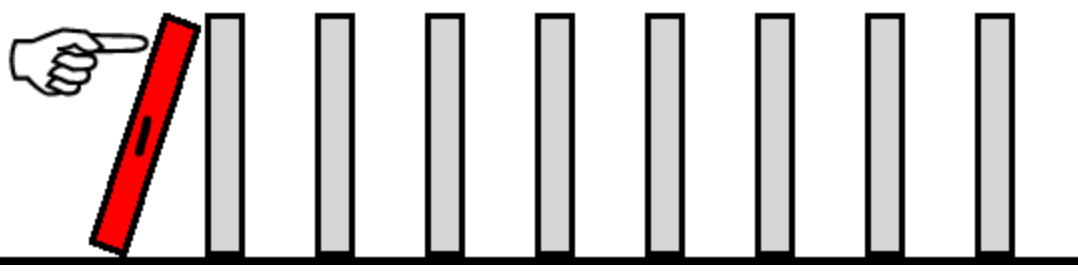
\includegraphics[scale=0.5]{InductionDominoes}
\end{center} 
% \vspace{-20pt}

Suppose we know the following: 

	\vspace{.2cm}
	\begin{enumerate}
	\item Domino \underline{\hspace{1cm}} falls

	\vspace{.25cm}
	\item If dominoes $1, 2, 3, \ldots , k$ \ ALL fall, then domino \underline{\hspace{1.5cm}} also falls (for any positive integer $k$)
	\end{enumerate}

\vspace{.5cm}
\textbf{Outcome:} Then, \underline{\hspace{2cm}} dominoes will fall!
\vspace{.25cm}   
}}
%%% end box



\vspace{.25cm}
%%%% something in a box
\noindent\fbox{%
\parbox{\textwidth}{\vspace{.25cm}
\hspace{5cm} \textbf{Principle of Strong Mathematical Induction} 

\vspace{.25cm}
To prove a statement, $P(n)$, is true for all integers $n \geq 1$ ($n \in \mathbb{Z}^+$), using \DarkPurple{strong induction}, there are 2 steps:

	\vspace{.5cm}
	\begin{enumerate}
	\item \MediumGreen{(Base Step):} Show \underline{\hspace{1.5cm}} is true \hspace{.5cm} (sometimes there is more than one base step)

	\vspace{.25cm}
	\item \MediumGreen{(Inductive Step):} Assume $P(1), P(2), P(3), \ldots , P(k)$ are ALL true for an arbitrary $k \in \mathbb{Z}^+$, and show this implies 

	\vspace{.25cm}
	that \underline{\hspace{1.75cm}} is true. 

    \vspace{.5cm}
    Another way to word this is to say: ``assume $P(j)$ is true for any integer $j$ such that $1 \leq j \leq k$, and show this implies that $P(k+1)$ is true"

%	\vspace{.25cm}
%	\hspace{1cm} i.e. show $\displaystyle{ \Big( P(1) \land P(2) \land \ldots \land P(k) \Big) \rightarrow \underline{\hspace{1.75cm}} }$
	\end{enumerate}
\vspace{.25cm}   
}}
%%% end box

\vspace{.5cm}

\subheader{Practice Problems}


\vspace{.25cm}


\begin{enumerate}

\item Prove that $3$ divides $n^3+2n$ whenever $n$ is a positive integer.

%%%
\newpage


\hspace{1cm}
\vspace{8cm}

\item What is wrong with this induction ``proof?" 

\vspace{.5cm}
\hspace{2cm} ``Theorem:" \hspace{.25cm} For every positive integer $n$, $\displaystyle{1+2+3+ \ldots + n = \frac{(n+\frac{1}{2})^2}{2} }$. 

\vspace{.5cm}
% \textbf{Base Step:} The formula is true for $n=1$. \\ \\
Let $P(k)$ be the statement: $\displaystyle{1+2+3+ \ldots + k = \frac{(k+\frac{1}{2})^2}{2} }$

\vspace{.25cm}
\textbf{Inductive Hypothesis:} We will assume that $P(k)$ is true, namely that $\displaystyle{1+2+3+ \ldots + k = \frac{(k+\frac{1}{2})^2}{2} }$

\vspace{.5cm}
We want to show that $P(k+1)$ is true, so we are trying to show that 

\vspace{.25cm}
    \hspace{1cm} $\displaystyle{1+2+3+ \ldots + k + (k+1) = \frac{(k+1+\frac{1}{2})^2}{2} }$

\vspace{.5cm}

Suppose that $\displaystyle{1+2+3+ \ldots + k = \frac{(k+\frac{1}{2})^2}{2} }$. Then, $\displaystyle{1+2+3+ \ldots + k + (k+1) =  \Big(1+2+3+ \ldots + k\Big) + k+1 }$. By the inductive hypothesis, we have that 

\vspace{.25cm}
$\displaystyle{1+2+3+ \ldots + k + (k+1) = \frac{(k+\frac{1}{2})^2}{2} + k + 1 = \frac{k^2+k+\frac{1}{4}}{2} + k + 1 = \frac{k^2+3k+\frac{9}{4}}{2} = \frac{(k+\frac{3}{2})^2}{2} = \frac{[(k+1) + \frac{1}{2}]^2}{2} }$, completing the inductive step. 


%%%
\newpage 

\item The NBA All-Star game experiments with a new long distance shooting contest where 40ft shots count 5pts and 50ft shots count 6pts. These are the only ways to earn points. For example, if Steph Curry makes three 40ft shots and two 50ft shots, he scores $3(5)+2(6)=27$ points. 
	\begin{enumerate}
	\item Find the largest integer $x$ such that a total score of $x$ points is \textbf{impossible}. 
	\item Prove that for all integers $n$ with $n \geq x+1$, a player can score $n$ points.
	\end{enumerate}


%%%
\newpage

\item Let $f_n$ be the $n$th Fibonacci number, defined by $f_0=0$, $f_1=1$ and $f_n=f_{n-1}+f_{n-2}$ for $n \geq 2$. Prove that $f_n \leq 2^n$ for all nonnegative integers. 

\vspace{.25cm}
\textbf{Note}: Since there are two ``initial values'' for this recursively defined sequence, we would need two base cases (regardless of whether we do weak induction or strong induction). 



\end{enumerate}




\end{document}





%%%% something in a box
\noindent\fbox{%
\parbox{\textwidth}{\vspace{.25cm}
\textbf{Strategies to Show Inductive Step}

\vspace{.25cm}
	\begin{enumerate}
	\item Start with $P(k)$ and do stuff to \underline{\hspace{4cm}} so it becomes $P(k+1)$

	\vspace{.25cm}
	\item Start with one side/part of $P(k+1)$ and use the assumption that \underline{\hspace{4cm}} to get the rest of $P(k+1)$
	\end{enumerate}
\vspace{.25cm}   
}}
%%% end box




\begin{multicols}{5} 
Type 
\columnbreak 

Symbol 
\columnbreak

Definition 
\columnbreak

\hspace{1cm}
 \columnbreak
 
\hspace{1cm}
\end{multicols}






%%%%%%%%%%%%%%%%%%%%%%%%%%%%%%%%%%%%%%%%%%%%%%%%%%%%%%%%%




%image aligned
%%
\includegraphics[scale=0.7, right]{BlankAxes}
\vspace{-10pt}


%image centered
%%
\begin{center}
\includegraphics[scale=1.4]{SinCosTanDrawGraphs}
\end{center} 
\vspace{-20pt}



%%% incorrect/correct show something with 2 approaches
\vspace{.25cm} 
\begin{multicols}{2} 
\red{\underline{Incorrect}} \columnbreak

\MediumGreen{\underline{Correct}} 
\end{multicols}


%%% Scratch work for proof
\hspace{7cm} \MediumGreen{\underline{Scratch Work}}
\begin{multicols}{2} 
\hspace{4cm} \MediumGreen{\underline{Given/Know}} \columnbreak

\MediumGreen{\underline{Want to show}} 
\end{multicols}

\vspace{2.5cm} 



%%%% something in a box
\noindent\fbox{%
\parbox{\textwidth}{\vspace{.25cm}
\textbf{Def:} \\ (1) The \DarkPurple{intersection} of sets $A$ and $B$ is the set of all elements in \textbf{both} $A$ \textbf{and} $B$, denoted $\underline{\hspace{2cm}}$. 
\vspace{.25cm}   
}}
%%% end box


%%% big row reduction arrow
\xrightarrow{\hspace*{2cm}}  



%%% table with extra vertical spacing
\begin{tabular}{ c|c|c } 
$f'(x)$ &  $f(x)$  &  $F(x)$  \\ \hline
\rule{0pt}{3ex}           &  $x^n$  &             \\
 \rule{0pt}{5ex}          &  $\displaystyle{x^{-1}=\frac{1}{x}}$   &             \\
\rule{0pt}{5ex}           &  $e^x$  &             \\
\rule{0pt}{5ex}           &  $e^{kx}$  &             \\
\rule{0pt}{5ex}           &  $g(x) \pm h(x)$  &             \\
\rule{0pt}{5ex}           &  $cg(x)$  &             \\
\rule{0pt}{5ex}           &  $g(x)h(x)$  &             \\
\rule{0pt}{5ex}           &  $\displaystyle{\frac{g(x)}{h(x)}}$  &             \\
\end{tabular}



%%% coefficient matrix template
$A = \mat{ 1 & 0 & 1 & 2 & 2 \\ 0 & 0 & 1 & 0 & 1 \\ 2 & 0 & 1 & 4 & 3 }$


%%% augmented matrix template (the number in brackets indicates which column the augmented bar will be placed AFTER)
$\begin{amatrix}{5}
1 & -1 & 0 & -5 & 0 & -9  \\ 
0 & 0  & 1 &  4 & 0 & 4 \\ 
0 & 0  & 0 &  0 & 1 & 3  
 \end{amatrix}$
 
 
 
 %%%% template for multiple alignment points in system of equations
 $\begin{alignedat}{3}
		x_1 &+ x_2 &&- x_3 &&= -6 \\
		3x_1 &+ x_2 &&+x_3  &&= 8 \\
		4x_1 &+ 2x_2 &&      &&= 2 \\
		\end{alignedat}$
